\documentclass{article}

\usepackage{fullpage}
\usepackage{graphicx}
\usepackage{hyperref}

\begin{document}

\begin{flushright}
    Jason Leung (jasleung)\\
    Christopher Oo (coo)\\
    Jacob Perrin (tcperrin)\\
    Alec Ten Harmsel (talec)
\end{flushright}

\begin{center}
    {\Huge
        EECS 373 Project Proposal: SCARH
    }
\end{center}

\section{High Level Description}
Our project is a soil monitoring system optimized for both size and power
consumption.  This is a project idea suggested by Professor Dutta as a research
project. The system will consist of an optimized sensor package and a base
station. The sensor package will take periodic measurements of the soil
moisture and temperature; this data will then be transmitted to a base station
for analysis and human interaction. The goal of the sensor system will be to
accurately and efficiently transmit data about the soil environment. At
minimum, the soil data will include temperature and moisture content data. In
addition to a sensor system, an accompanying base station will retrieve the
data and display it in a human-understandable format as well as transferring it
to the cloud to be stored permanently and analysed further. This base station
will have LED indicators indicating the current moisture content of the soil,
as well as potentiometers to set the allowable bounds for acceptable moisture
content.

\section{Project Functionality}

\begin{itemize}
    \item Soil moisture sensing
        \begin{itemize}
            \item Generate a 100kHz sine wave
            \item Measure the phase delay to derive the capacitance of the
                soil.  The water content is the largest factor contributing to
                the soil's capacitance.
        \end{itemize}
    \item Temperature sensing
        \begin{itemize}
            \item Use a temperature sensor to sense soil temperature
        \end{itemize}
    \item Data display
        \begin{itemize}
            \item Sensor data will be recorded and transmitted to the base
                station
            \item Base station will receive data, calculate values based on a
                calibration curve, and display the data in a human readable way
                as well as transmit the data to the cloud for further
                processing
        \end{itemize}
    \item Low power without batteries
        \begin{itemize}
            \item A solar power system will supply power to the entire sensing
                system
            \item Periodic updates will be collected on a standard interval
            \item Timer-based interrupt-driven wakeup signal from lower-power
                standby mode
        \end{itemize}
\end{itemize}

\subsection{Input Devices}
\begin{itemize}
    \item ADC
    \item Temperature sensor
	\item BLE receiver
	\item Potentiometer
\end{itemize}

\subsection{Output Devices}
\begin{itemize}
	\item DAC
    \item BLE transmitter
	\item Ethernet
	\item Status LEDs (Sensor)
	\item Status LEDs (Receiver)
	\item LCD display
\end{itemize}

\subsection{Complexities}
\begin{itemize}
    \item Power optimization
        \begin{itemize}
            \item Optimize standby and active power consumption
            \item Minimize on-board processing
        \end{itemize}
    \item Physical size optimization
        \begin{itemize}
            \item Minimize physical footprint
            \item Manage tradeoff between solar cell area and supplied power
        \end{itemize}
    \item Design moisture sensor
        \begin{itemize}
            \item Design calibration process and algorithm
            \item Design data acquisition method (ADC/DAC) with on-board
                statistical analysis
            \item Design physical probing system
        \end{itemize}
    \item Lab skills
        \begin{itemize}
            \item Bus interfacing with SPI and I2C
            \item Device Driver with BLE receiver
            \item Interrupts
            \item General Purpose Timers
            \item Analog to Digital (ADC) and Digital to Analog (DAC)
        \end{itemize}
\end{itemize}

\subsection{Difficulty Components}
\begin{itemize}
    \item Custom PCB
    \item Custom moisture sensor (ADC/DAC)
    \item BLE radio transmitter/receiver
    \item Temperature sensor
    \item Solar cell
	\item Ethernet controller
	\item Potentiometer-based calibration
	\item LCD display
\end{itemize}

\section{Functional Block Diagram}
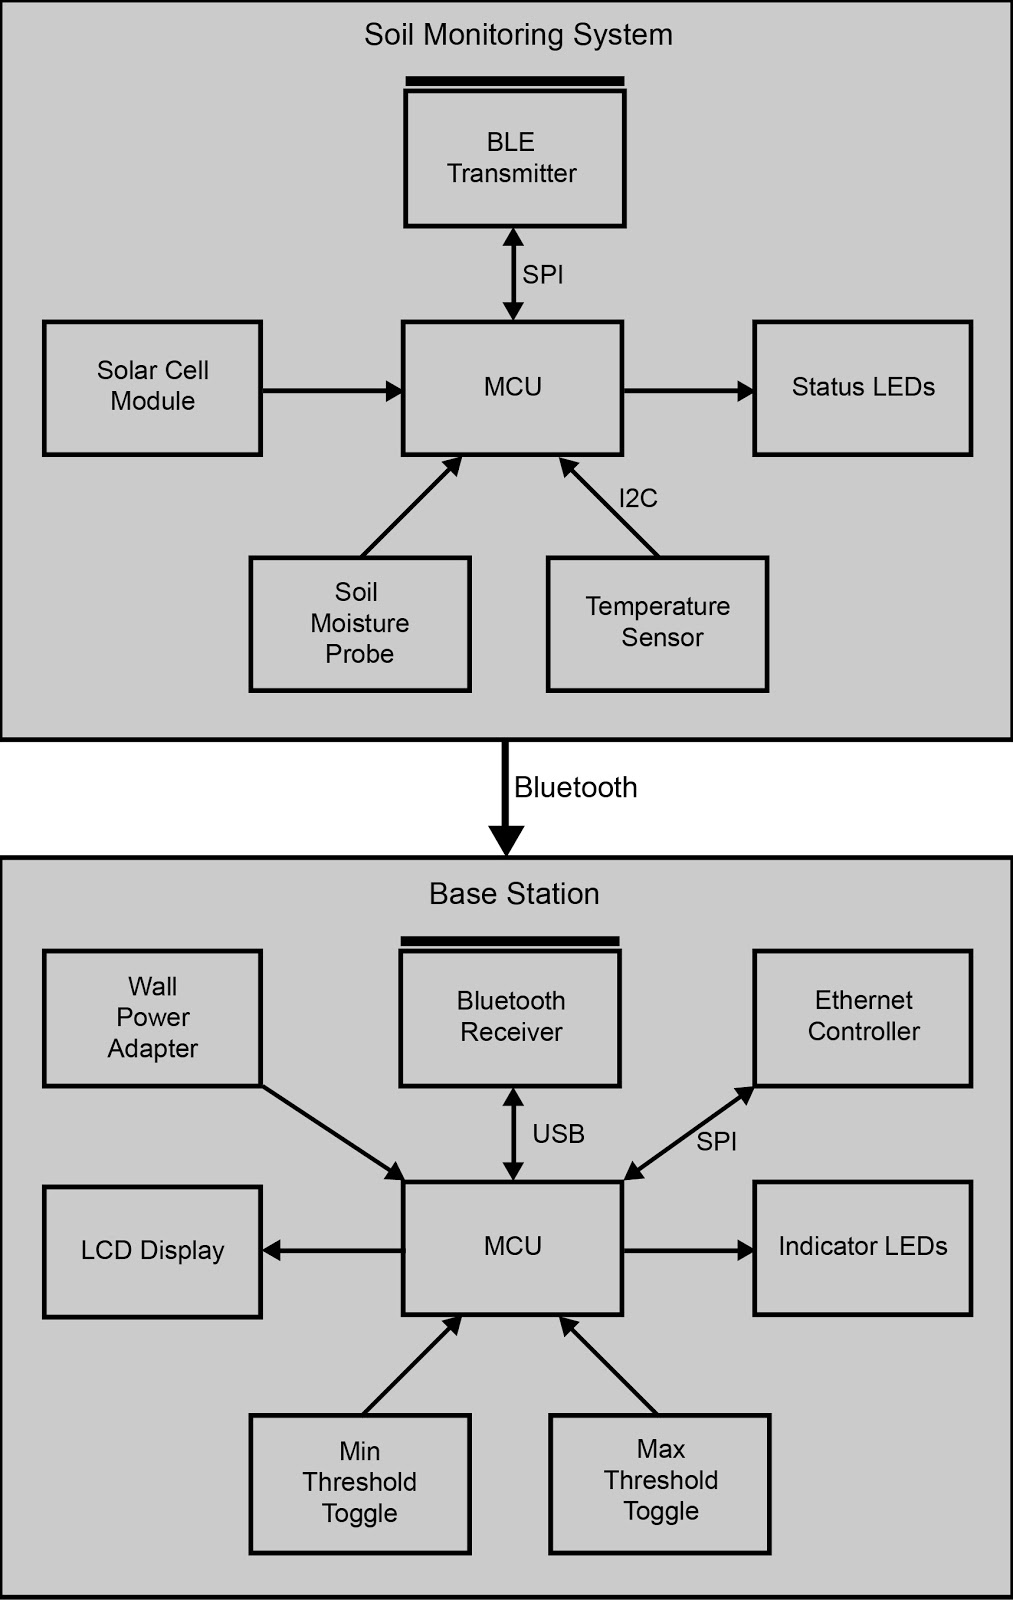
\includegraphics[width=0.9\textwidth]{functional_diagram.png}

\section{Component Level Diagram}
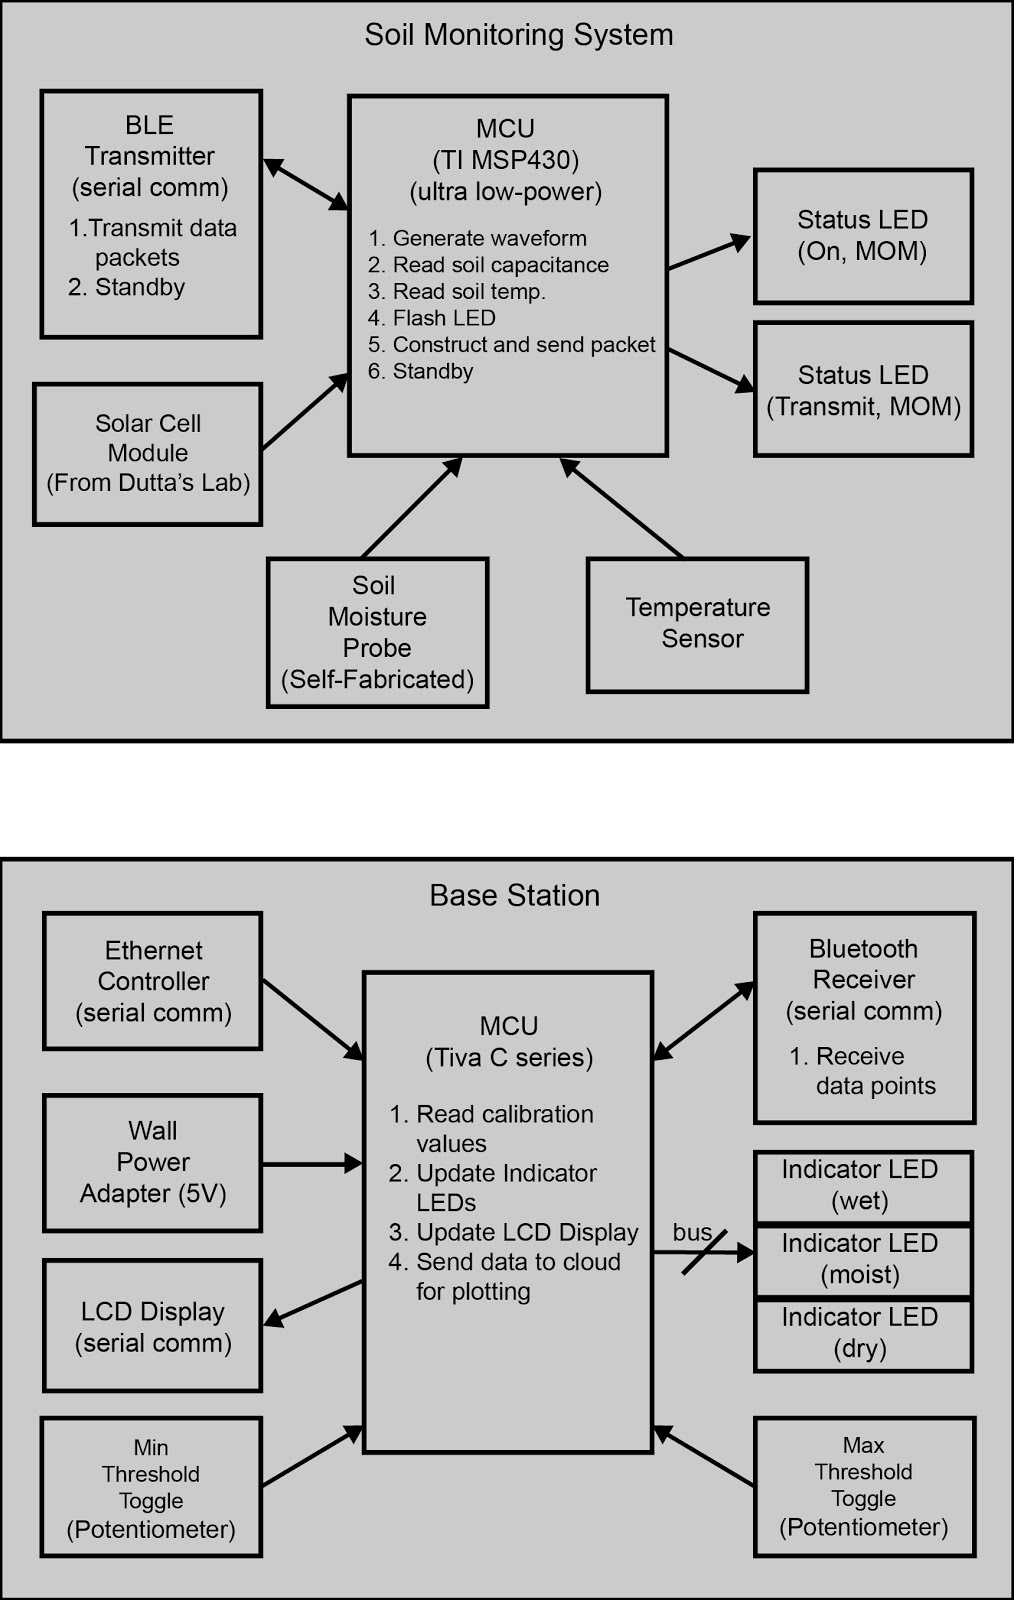
\includegraphics[width=0.9\textwidth]{component_diagram.png}

\section{Preliminary Component List}
\begin{itemize}
    \item Sensor Package
        \begin{itemize}
            \item Microcontroller: TI MSP430L09x
                \url{http://www.ti.com/lsds/ti/microcontrollers_16­bit_32­bit/msp/ultra­low_powe
                r/msp430l09x_low_voltage/overview.page}
            \item BLE radio: Nordic nRF8001
                \url{http://www.nordicsemi.com/eng/Products/Bluetooth­R­low­energy/nRF8001}
            \item Tempurature Sensor: TI TMP102 http://www.ti.com/product/tmp102
            \item Solar Cell: ~20x BPW34 https://www.sparkfun.com/products/9541
            \item Soil Probe: Custom built and designed PCB
            \item LEDs ­ Amber and Green variants, low current draw:
                \url{http://www.digikey.com/short/787w0q}
        \end{itemize}
    \item Base Station: 
        \begin{itemize}
            \item BLE Radio receiver provided by Prof. Dutta
            \item Tiva C Series microcontroller:
                \url{http://www.ti.com/lit/ds/symlink/tm4c1294ncpdt.pdf}
                FPU allows for easy floating point computation
            \item
                (Alternatively) Laptop computer/Raspberry Pi for data analysis
            \item LCD Display: \url{https://www.sparkfun.com/products/10168}
            \item
                LEDs ­ Red and Green variants:
                \url{http://www.digikey.com/short/787wdd}
            \item 5V wall power adapter:
                \url{https://www.sparkfun.com/products/8269}
            \item Potentiometers: \url{https://www.sparkfun.com/products/9939}
            \item
                Ethernet controller module: \url{https://www.sparkfun.com/products/765}
                or just the controller chip: \url{http://www.digikey.com/short/787n73}
                \url{http://dlnmh9ip6v2uc.cloudfront.net/datasheets/BreakoutBoards/39662b.pdf}
        \end{itemize}
\end{itemize}

\end{document}
